\documentclass[11pt]{article}
\usepackage[utf8]{inputenc}
\usepackage[margin=.9in]{geometry}

\usepackage{qtree}

\usepackage{algorithm}
\usepackage[noend]{algpseudocode}
\algnewcommand\Or{\textbf{ or }}
\algnewcommand\And{\textbf{ and }}
\usepackage{graphicx}
\usepackage{enumitem}
\usepackage{hyperref}

\usepackage{tikz}
\usetikzlibrary{calc,shapes.multipart,chains,arrows,positioning}
\tikzstyle{vertex}=[draw,fill=myseagreen,circle,minimum size=24pt,inner sep=0pt]
\definecolor{myseagreen}{RGB}{240,240,240}
\definecolor{mysalmon}{RGB}{240,180,170}

\title{Segment Trees}
\author{Richard Zhan\footnote{Based on George Tang/Justin Zhang's Segment Tree lecture}}
\date{November 2019}

\begin{document}

\maketitle
\section{Introduction}
Given a list of data, efficiently process the following range queries across any interval:

\begin{itemize}
    \item Find the sum
    \item Find the min/max
    \item Add a value to each element
\end{itemize}

A \textit{segment tree} is a powerful data structure for storing intervals, or \textit{segments}. Segment trees can efficiently answer dynamic range queries. We will use a segment tree to solve the Range Minimum Query (RMQ) problem and the Range Sum Query (RSQ), which is the problem of finding the minimum element/sum of elements in an array within a given range $i$ to $j$. Other range queries include range GCD, or product, and more. Moreover, all of our segment trees will support interval updates.

\section{Construction}
A segment tree is a balanced binary tree in which each leaf represents an element in the array. The root of the tree represents segment $[0, n-1]$, and for each segment$[l, r]$ represented by the node at index $p$, the left child represents the segment $[l, (l + r) / 2]$ and the right child represents the segment $[(l + r) / 2 + 1, r]$. In the case of RMQ, ``represents" means the value of the node is the minimum of the segment it represents. For example, for the array $[-1, 3, 4, 0, 2, 1]$, the tree would look as follows:

\Tree [.-1 [.-1 [.-1 -1 3 ] 4 ] [.0 [.0 0 2 ] 1 ]]

\medskip
Constructing this tree takes $O(n)$ time and $O(n)$ space. In the pseudocode below, we build the tree recursively. The tree is represented as an array $st$ where index 1 is the root of the tree and the left and right children of index $p$ are indices $2 \times p$ and $(2 \times p) + 1$, respectively. $l$ and $r$ are the left and right bounds of the current segment, respectively.

Note, however, that we can construct this tree by updating length-one ranges $n$ times. This gives us a runtime of $O(n \log n)$ for construction, which is usually fast enough.

\begin{algorithm}[H]
\caption{Segment Tree Construction}
\begin{algorithmic}
    \Function{Build}{$p$, $l$, $r$}
        \If {$l = r$}
            \State $st[p] \gets A[l]$
        \Else
            \State $pl \gets 2 \times p$
            \State $pr \gets 2 \times p + 1$
            \State $\Call{Build}{pl, l, (l + r) / 2}$
            \State $\Call{Build}{pr, (l + r) / 2, r}$
            \State \Return $\Call{min}{st[pl], st[pr]}$
        \EndIf
    \EndFunction
\end{algorithmic}
\end{algorithm}

\section{Solving Queries}

There are three cases that we must consider when traversing a segment tree: when part of the segment represented by the node is within the query; when the segment is completely within the query; and when the segment is completely outside of the query. If part of the segment is within the query, we must check both of the node's children. If the segment is completely within the query, we return the node's value, which is the minimum of the segment it represents. If the segment is completely outside of the query, we return some very large number. In the pseudocode below, we traverse the tree recursively. 

With the segment tree built, solving queries takes $O(\log n)$ time. This is because segment trees allow us to avoid traversing unrelated parts of the tree. In the worst case, in which only part of every segment we reach is within the query, we traverse two root-to-leaf paths, taking $O(2 \times \log n) = O(\log n)$ time.

\begin{algorithm}[H]
\caption{Range Minimum Query Using a Segment Tree}
\begin{algorithmic}
    \Function{RMQ}{$p$, $l$, $r$, $i$, $j$}
        \If {$i > r \Or j < l$}
            \State \Return $\infty$
        \EndIf
        \If {$l >= i \And r <= j$}
            \State \Return $st[p]$
        \EndIf
        \State $pl \gets 2 \times p$
        \State $pr \gets 2 \times p + 1$
        \State $minl \gets \Call{RMQ}{pl, l, (l + r) / 2, i, j}$
        \State $minr \gets \Call{RMQ}{pr, (l + r) / 2 + 1, r, i, j}$
        \State \Return $\Call{min}{minl, minr}$
    \EndFunction
\end{algorithmic}
\end{algorithm}

\begin{algorithm}[H]
\caption{Range Sum Query Using a Segment Tree}
\begin{algorithmic}
    \Function{RSQ}{$p$, $l$, $r$, $i$, $j$}
        \If {$i > r \Or j < l$}
            \State \Return $0$
        \EndIf
        \If {$l >= i \And r <= j$}
            \State \Return $st[p]$
        \EndIf
        \State $pl \gets 2 \times p$
        \State $pr \gets 2 \times p + 1$
        \State \Return $\Call{RSQ}{pl, l, (l + r) / 2, i, j} + \Call{RSQ}{pr, (l + r) / 2 + 1, r, i, j}$
    \EndFunction
\end{algorithmic}
\end{algorithm}

\section{Lazy propagation}
With a segment tree, we can handle \textit{point updates}, or updates of individual elements in $log(N)$ time (find leaf node and recurse up). But what if we also wanted to perform \textit{range updates}, or updates of a range of elements? If we want to increment the value of $m$ contiguous elements, this will take $O(m \log n)$ time.

Fortunately, we can do better. With our current data structure, performing a range update will require modifying the values of $m$ elements, so we need to change our data structure. To avoid recursing all the way to the bottom of the tree for all $m$ elements, we can store some information in higher nodes instead.

Let's say we're performing a range update on the range $u$, and we're examining the segment $s$. The key insight is that if $s$ is contained within $u$, then we can simply set a \textit{lazy} value for $s$ instead of recursing on its children. When a lazy value is set, it means that the values of \textbf{each of} the children of that node should be incremented by that value.

\begin{figure}[h]
\center
{
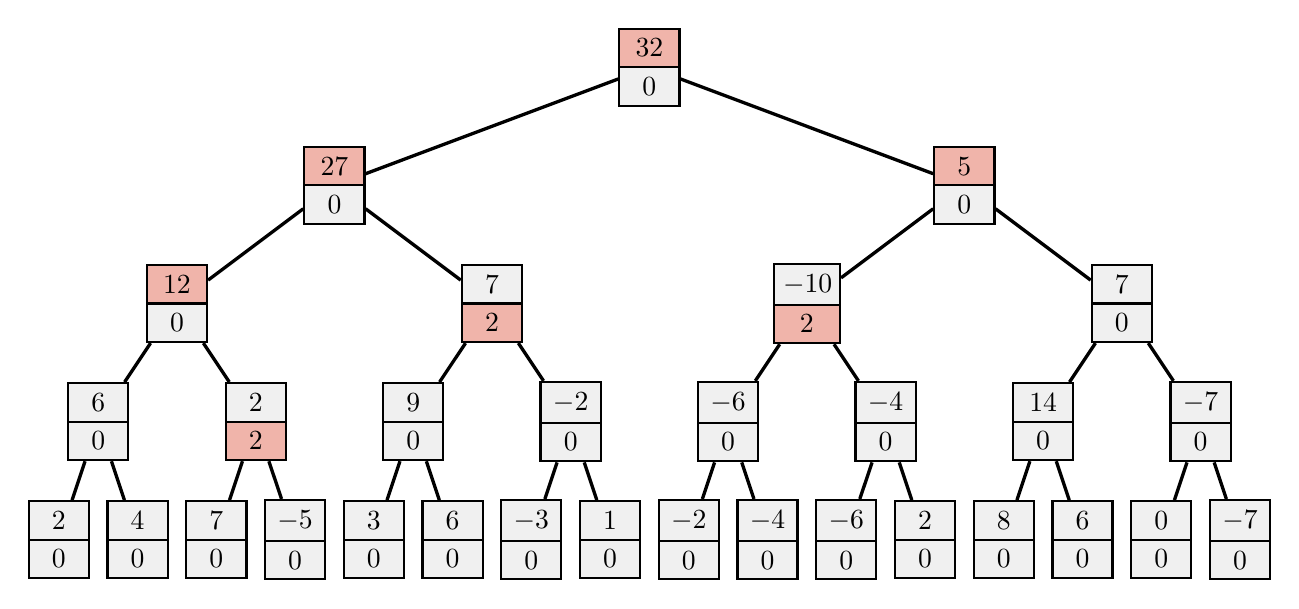
\begin{tikzpicture}[
  very thick,
  level 1/.style={sibling distance=80mm},
  level 2/.style={sibling distance=40mm},
  level 3/.style={sibling distance=20mm},
  level 4/.style={sibling distance=10mm},
  myrect/.style={
    draw,
    thick,
    rectangle split,
    rectangle split parts=2,
    rectangle split part fill={myseagreen, myseagreen},
    rectangle split part align=left,
    text width=3.5ex,
    text centered
    }
]
\node [myrect, rectangle split part fill={mysalmon, myseagreen}] (r){$32$\nodepart{two}0}
  child {
    node [myrect, rectangle split part fill={mysalmon, myseagreen}] (a) {27\nodepart{two}0}
    child {
      node [myrect, rectangle split part fill={mysalmon, myseagreen}] {12\nodepart{two}0}
      child {
        node [myrect] {6\nodepart{two}0}
        child {node [myrect] {2\nodepart{two}0}}
        child {node [myrect] {4\nodepart{two}0}}
      } 
      child {
        node [myrect, rectangle split part fill={myseagreen, mysalmon}] {2\nodepart{two}2}
        child {node [myrect] {7\nodepart{two}0}}
        child {node [myrect] {$-5$\nodepart{two}0}}
      }
    }
    child {
      node [myrect, rectangle split part fill={myseagreen, mysalmon}] {7\nodepart{two}2}
      child {node [myrect] {9\nodepart{two}0}
              child {node [myrect] {3\nodepart{two}0}}
        child {node [myrect] {6\nodepart{two}0}}
      }
      child {node [myrect] {$-2$\nodepart{two}0}
              child {node [myrect] {$-3$\nodepart{two}0}}
        child {node [myrect] {1\nodepart{two}0}}
      }
    }
  }
  child {
    node [myrect, rectangle split part fill={mysalmon, myseagreen}] {$5$\nodepart{two}0}
    child {
      node [myrect, text width=4ex, rectangle split part fill={myseagreen, mysalmon}] {$-10$\nodepart{two}2}
      child {node [myrect] {$-6$\nodepart{two}0}
              child {node [myrect] {$-2$\nodepart{two}0}}
        child {node [myrect] {$-4$\nodepart{two}0}}}
      child {node [myrect] {$-4$\nodepart{two}0}
              child {node [myrect] {$-6$\nodepart{two}0}}
        child {node [myrect] {$2$\nodepart{two}0}}}
    }
    child {
      node [myrect] {7\nodepart{two}0}
      child {node [myrect] {14\nodepart{two}0}
              child {node [myrect] {8\nodepart{two}0}}
        child {node [myrect] {6\nodepart{two}0}}}
      child {node [myrect] {$-7$\nodepart{two}0}
              child {node [myrect] {0\nodepart{two}0}}
        child {node [myrect] {$-7$\nodepart{two}0}}}
    }
  };

\end{tikzpicture}
}
\caption{Example of a segment tree with lazy values stored underneath. The highlighted values reflect the values updated after calling $update(3, 12, 2)$. \textit{Credit: Samuel Hsiang.}}
\end{figure}

However, if we encounter a lazy value while performing a query or an update, however, we need to push the value by moving the lazy value into its children, and updating the current node's sum correspondingly. But because we only push once per node, these operations still only take $O(\log n)$.

We can also use this technique to implement the range minimum query (RMQ) problem. A full implementation of both is provided by the solution to Counting Haybales (USACO December 2015, Platinum) at \url{http://www.usaco.org/current/data/sol_haybales_platinum_dec15.html}.

\section{Lattices and Segment Trees}
Segment trees can be applied in 2 dimensional geometric problems. Imagine a 2D grid composed on points, where each have a specific value. Now image a line sweeping across it, and at every instance we are asked about the points that have already been 'seen'. Segment trees allow us to quickly determine the properties of 'seen' points.

\subsection{Why Did the Cow Cross the Road II, USACO 2017 Platinum}
We can start at any lattice point, and we can move to another lattice point if and only if that lattice point has x and y coordinates that strictly exceed that of the point we are currently at. We wish to compute the maximum number of lattice points we can visit.

Each lattice points stores the maximum number of points that can be visited under the condition that it is the last lattice point visited. As we move to a new lattice points, we insert all lattice points we just encountered at the instance into the segment trees (intervals are based on y value), and query the max of those points that have y value less than that of the current point (range = [0, y]).  


\section{Problems}
\begin{enumerate}
    \item Counting Haybales (see link above)
    \item You're given an array of length $10^5$, consisting of $0$'s and $1$'s. Answer $10^5$ operations, where each operation is either to invert the bits from a given $i$ to $j$ or to count the number of set bits from $i$ to $j$.
    \item You're given an array $t$ of length $2^{17}$, with non-negative integers less than $2^{30}$. Let's define an OR($a$) to be the result after bitwise-OR'ing pairs of elements in an array $a$ (OR($a$) := {a[1] OR a[2], a[3] OR a[4], ...}) and XOR($a$) to be the result after bitwise-XOR'ing pairs of elements in an array $a$ (XOR($a$) := {a[1] XOR a[2], a[3] XOR a[4], ...}). V($a$) is then defined to be the final value after alternating the OR and XOR operations (beginning with OR) on an array $a$ until there is one value left: OR(XOR(OR(XOR(...OR(a)...)))). Answer $10^5$ operations, where each operation sets the value of $t$ at index $i$ to a new value and then calculates V($t$) (Codeforces 339D).
    \item You're given an array of length $10^5$. Answer $5 \times 10^4$ queries, where each query either asks to print the sum of all elements from a given index $l$ to a given index $r$ or to apply a bitwise-XOR to all elements between $l$ and $r$ with a value $x$ (Codeforces 242E).
\end{enumerate}

\end{document}
